\setcounter{chapter}{1}
\chapter{\label{sec:data}\g12 Data Acquisition \& Reconstruction}

A raw event collected by the data acquisition (\abbr{DAQ}, see Sec.~\ref{sec:clas.daq}) consisted of many hundreds of ``hits'' corresponding to signals from the detector that were strong enough to be recorded, that is, above a certain threshold. The hits paired detector element identification numbers with either an \abbr{ADC} or \abbr{TDC} value. These were converted to manageable units in energy for \abbr{ADC}s, time for \abbr{TDC}s and sector/wire number for the element \abbr{ID}s. After that, these hits were grouped into ``clusters'' which eventually represented measured particles that had traveled through the detector. This process, called \emph{reconstruction}, is detailed in the following sections and starts with the definition of the ``trigger'' that told the \abbr{DAQ} to record an event.

The \emph{main production trigger} used by the \g12 experiment was a coincidence of two charged tracks in different sectors and at the same time as a tagged photon above 4.4~GeV. These tracks were identified at the trigger level by the coincidence of a start counter hit and a time-of-flight hit in the same sector as identified by ``\abbr{ST$\times$TOF}'' in Fig.~\ref{fig:clas.daq.trigsec}. With an electron beam current of 60--65~nA, the \abbr{DAQ} rate was approximately 8~kHz with the two-track trigger contributing approximately 5.5~kHz to this total. All trigger \emph{bits} used during \g12, numbered 1--12, can be found in Tables~\ref{tab:data.trig.conf.1}, \ref{tab:data.trig.conf.2} and \ref{tab:data.trig.conf.3}.

Several lower-rate triggers were used in addition to the main production trigger. Of special note was bit 6: a single lepton in coincidence with a single charged track. This trigger matched hits in the electromagnetic calorimeter with the \v{C}erenkov counter, both above certain thresholds as discussed below. It is designated by ``\abbr{EC$\times$CC}'' in Table~\ref{tab:data.trig.conf.2}, and overlapped with the production trigger adding approximately 1~kHz to the \abbr{DAQ} rate. Also of note, bit 12 was a three-track coincidence without requiring an in-time tagger hit (see Sec.~\ref{sec:clas.tagr}) contributing an additional 1~kHz.

The \g12 experiment incorporated several runs which consisted of lower current ($\sim24$~nA), single track triggers. These were part of a late proposal\cite{clas.proposal.pion}, led by the Duke University group, as discussed in Sec.~\ref{sec:clas.g12} on page \pageref{sec:clas.g12}. Also, Several calibration and normalization runs were taken throughout the experiment as shown in Table~\ref{tab:data.calibruns}. For this analysis, these were used largely for alignment corrections and the total photon flux determination.

The raw data recorded from the \abbr{CLAS} detector consisted of \abbr{ADC} and \abbr{TDC} signals from the individual elements of each subsystem. The data also included scalar values from the accelerator such as the \abbr{RF} clock, which had the best timing resolution of all signals. Reconstruction of tracks from these element hits started by spatially grouping the drift-chamber (\abbr{DC}) hits into \emph{hit-based} candidate tracks and then refining these using the timing from the start (\abbr{ST}) and time-of-flight (\abbr{TOF}) counters. Particle identification was then done on these tracks by several means including mass determination and energy deposit as discussed later in this chapter. Neutral particles that did not fire the \abbr{DC} (photons, for example) were identified by certain signatures in the electromagnetic calorimeter (\abbr{EC}), though the efficiency for detecting neutral particles was much lower than for charged particles.

The tracks which were the result of reconstruction consisted primarily of momentum and vertex information. Timing from the \abbr{TOF} and \abbr{ST} were used during analysis to fine-tune the particle identification. This chapter discusses the reconstruction of tracks from raw data, the resolution of the momenta and timing information, and finally, a technical itemization of the variables used in the analysis of this work, and their inter-relationships.

\section{\label{sec:data.runsum}Run Summary}

The \g12 experiment is divided into several ``runs,'' each consisting of approximately 50 million triggers. Calibrations were largely determined and applied based on run number or a specific range of runs. Table~\ref{tab:data.cook.prodruns} contains a list of the runs that had at least 1M triggers and were reconstructed successfully, along with the current of the beam for these runs. Table~\ref{tab:data.cook.singlesecruns} shows a list of the single-sector runs taken throughout the \g12 running period. Data from these runs represent approximately 97\% of the production running period of \g12. There were many diagnostic runs that were not recorded. Most of these involved testing the \abbr{DAQ} system, however, the run number still incremented for each of these. Further complicating matters, several files did not have adequate information for the reconstruction process due to hardware failures during periods where the \abbr{DAQ} was active and data was being written to disk --- wire tripping in the \abbr{DC}, for example. In the end, the \g12 experiment consisted of 622 ``good'' runs starting with 56363 and ending with 57317.

\small
\begin{center}
\begin{singlespacing}
\begin{longtable}{lr|lr|lr|lr}
\caption[Production Run List]{\label{tab:data.cook.prodruns}List of successfully reconstructed production runs and their beam currents in nA.} \\

\hline \hline
\multicolumn{2}{l|}{runs} & \multicolumn{2}{l|}{runs} & \multicolumn{2}{l|}{runs} & \multicolumn{2}{l}{runs} \\
\multicolumn{2}{r|}{current (nA)} & \multicolumn{2}{r|}{current (nA)}  & \multicolumn{2}{r|}{current (nA)} & \multicolumn{2}{r}{current (nA)} \\
\hline
\endfirsthead

\multicolumn{8}{l}{\scriptsize continued from previous page.} \\
\hline
\multicolumn{2}{l|}{runs} & \multicolumn{2}{l|}{runs} & \multicolumn{2}{l|}{runs} & \multicolumn{2}{l}{runs} \\
\multicolumn{2}{r|}{current (nA)} & \multicolumn{2}{r|}{current (nA)}  & \multicolumn{2}{r|}{current (nA)} & \multicolumn{2}{r}{current (nA)} \\
\hline
\endhead

\hline
\multicolumn{8}{r}{\scriptsize continued on next page.} \\
\endfoot

\hline \hline
\endlastfoot

56363	&	20	&	56505-56506 	&	40	&	 56774-56778 	&	65	&	56958	&	60	\\
56365	&	30	&	56508-56510 	&	60	&	 56780-56784 	&	65	&	 56960-56975 	&	60	\\
56369	&	30	&	56513-56517 	&	60	&	 56787-56788 	&	65	&	 56977-56980 	&	60	\\
56384	&	5	&	56519	&	60	&	 56791-56794 	&	65	&	 56992-56994 	&	60	\\
56386	&	20	&	56521-56542 	&	60	&	 56798-56802 	&	65	&	 56996-57006 	&	60	\\
56400-56401 	&	50	&	56545-56550 	&	60	&	 56805-56815 	&	65	&	 57008-57017 	&	60	\\
56403	&	70	&	56555-56556 	&	60	&	 56821-56827 	&	65	&	 57021-57023 	&	60	\\
56404	&	60	&	56561-56564 	&	60	&	 56831-56834 	&	65	&	 57025-57027 	&	60	\\
56405	&	50	&	56573-56583 	&	60	&	 56838-56839 	&	65	&	 57030-57032 	&	60	\\
56406	&	40	&	56586-56593 	&	60	&	 56841-56845 	&	65	&	 57036-57039 	&	60	\\
56408	&	80	&	56605	&	60	&	56849	&	65	&	 57062-57069 	&	60	\\
56410	&	90	&	 56608-56612 	&	60	&	 56853-56862 	&	65	&	 57071-57073 	&	60	\\
56420-56422 	&	5	&	 56614-56618 	&	60	&	56864	&	65	&	 57075-57080 	&	60	\\
56435	&	5	&	 56620-56628 	&	60	&	 56865-56866 	&	60	&	 57095-57097 	&	60	\\
56436	&	15	&	 56630-56636 	&	60	&	56870	&	65	&	 57100-57103 	&	60	\\
56441	&	35	&	 56638-56644 	&	60	&	 56874-56875 	&	60	&	 57106-57108 	&	60	\\
56442	&	30	&	56646	&	60	&	56877	&	60	&	 57114-57128 	&	60	\\
56443	&	20	&	 56653-56656 	&	60	&	56879	&	60	&	 57130-57152 	&	60	\\
56445-56450 	&	60	&	 56660-56661 	&	60	&	 56897-56898 	&	60	&	 57159-57168 	&	60	\\
56453-56459 	&	60	&	 56665-56670 	&	60	&	56899	&	65	&	 57170-57185 	&	60	\\
56460-56462 	&	70	&	 56673-56675 	&	60	&	 56900-56908 	&	60	&	 57189-57229 	&	60	\\
56465	&	70	&	 56679-56681 	&	60	&	 56914-56919 	&	60	&	 57233-57236 	&	60	\\
56467-56472 	&	70	&	56683	&	60	&	 56921-56922 	&	60	&	 57249-57253 	&	60	\\
56478-56483 	&	70	&	 56685-56696 	&	60	&	56923	&	65	&	 57255-57258 	&	60	\\
56485-56487 	&	70	&	 56700-56708 	&	60	&	56924	&	70	&	 57260-57268 	&	60	\\
56489-56490 	&	70	&	 56710-56724 	&	60	&	56925	&	80	&	 57270-57288 	&	60	\\
56499	&	70	&	 56726-56744 	&	60	&	 56926-56930 	&	60	&	 57290-57291 	&	60	\\
56501	&	60	&	 56748-56750 	&	60	&	56932	&	60	&	 57293-57312 	&	60	\\
56503	&	57	&	 56751-56768 	&	65	&	 56935-56940 	&	60	&	 57314-57317 	&	60	\\
56504	&	56	&	 56770-56772 	&	65	&	 56948-56956 	&	60	&	  	&	  	\\

\end{longtable}
\end{singlespacing}
\end{center}
\vspace{20pt} % label:  tab:data.cook.prodruns

\begin{table}
\begin{minipage}{\textwidth}
\begin{center}
\begin{singlespacing}

\caption[Single-prong Run List]{\label{tab:data.cook.singlesecruns}A list of the single-prong runs using the trigger configuration described in Table~\ref{tab:data.trig.conf.3}.\vspace{0.75mm}}

\begin{tabular}{lr|lr}

\hline
run & current (nA) & run & current (nA) \\
\hline

56476 & 24 & 56910 & 35 \\
56502 & 24 & 56911 & 30 \\
56520 & 24 & 56912 & 25 \\
56544 & 24 & 56913 & 24 \\
56559 & 24 & 56933-56934 & 24 \\
56585 & 24 & 56981-56983 & 24 \\
%56619 & 24 & 56985\footnotemark{foot:no_l2} & 15 \\ 
56619 & 24 & 56985 & 15 \\
56637 & 24 & 56986 & 15 \\
56663-56664 & 24 & 56989 & 24 \\
56697 & 24 & 57028 & 24 \\
56725 & 24 & 57061 & 24 \\
56747 & 24 & 57094 & 24 \\
56769 & 24 & 57129 & 24 \\
56804 & 24 & 57155-57156 & 24 \\
56835 & 24 & 57237-57238 & 24 \\
56869 & 5 \\

\hline \hline

\end{tabular}

\end{singlespacing}
\end{center}
\end{minipage}
\end{table}
\vspace{20pt} % label:  tab:data.cook.singlesecruns

In addition to the production data taken, there were several special \emph{calibration} runs which are listed in Table~\ref{tab:data.calibruns}. These consisted of normalization, zero-field, and empty-target data. The normalization runs were used to calibrate the tagger for the measurement of the total photon flux and there were two specific runs for the left and right \abbr{TDC} signals of the tagger to check for consistency. The zero-field data was taken with the main torus magnet off. This meant that the particles traveled in straight lines through the drift-chamber which made track reconstruction simple and accurate. Though their momenta were unknown, these tracks were used to account for the position and orientation of the drift-cambers in the reconstruction. Finally, the empty target run was used to investigate the contributions of the target wall to the data sample.

\begin{center}
\begin{singlespacing}
\begin{longtable}{ccl}
\caption[\g12 Special Run List]{\label{tab:data.calibruns}List of special calibration runs done during the \g12 experiment.} \\

\hline
run & current (nA) & description \\
\hline
\endfirsthead

\multicolumn{3}{l}{\scriptsize continued from previous page.} \\
\hline
run & current (nA) & description \\
\hline
\endhead

\hline
\multicolumn{3}{r}{\scriptsize continued on next page.} \\
\endfoot

\hline \hline
\endlastfoot

56397 & 0.05 & normalization \\
56475 & 10 & zero-field \\
56511 & 0.05 & normalization \\
56512 & 0.05 & normalization \\
56584 & 0.05 & normalization \\
56682 & 0.05 & normalization \\
56790 & 0.05 & normalization \\
56931 & 0.05 & normalization \\
56947 & 0.05 & normalization \\
57169 & 0.05 & normalization \\
57239 & 24 & empty-target, single-sector \\
57241 & 80 & empty-target, production \\
57248 & 0.05 & normalization

\end{longtable}
\end{singlespacing}
\end{center}
\vspace{20pt} % label:  tab:data.calibruns

\section{\label{sec:data.trig}Trigger Configuration}

The \g12 experiment was the first Hall \desg{B} run-period to implement field programmable gate array (\abbr{FPGA}) processors to handle the trigger logic of the \abbr{CLAS} detector (see Sec.~\ref{sec:clas.daq}). With this new \abbr{FPGA}-powered triggering system, came the ability to modify the trigger quickly during the experiment. While potentially dangerous --- these changes must be accounted for in total-cross-sectional analyses for example --- this allowed the group to tune the trigger to get the highest possible rate of physical events.

The trigger bits used during the \g12 running period are defined in Tables~\ref{tab:data.trig.conf.1}, \ref{tab:data.trig.conf.2} and \ref{tab:data.trig.conf.3}. They generally consisted of a number of tracks which were the coincidence of any one of the four start counter paddles and any of the 57 time-of-flight paddles in a given sector as discussed in Sec.~\ref{sec:clas.daq}. The hardware and configuration did not allow triggering on two tracks in the same sector because there were only six signals coming from the \abbr{TOF} --- one for each sector. The coincidence of these tracks with the photon tagger, called the ``Master-\abbr{OR},'' is defined in Table~\ref{tab:data.trig.mor}.

\begin{table}
\begin{minipage}{\textwidth}
\begin{center}
\begin{singlespacing}

\caption[Trigger Configuration 1]{\label{tab:data.trig.conf.1}Trigger configuration for \g12 runs from 56363 to 56594 and 56608 to 56647. (\abbr{ST}$\cdot$\abbr{TOF})$_{i}$ indicates a trigger-level track defined as a coincidence between a start counter and time-of-flight hit in the \ith\ sector. \abbr{MORA} and \abbr{MORB} represent coincidences with tagger hits within a certain energy range as specified in Table~\ref{tab:data.trig.mor}.}

\begin{tabular}{cccc}

\hline

\multicolumn{4}{c}{\g12 runs 56363--56594, 56608--56647} \\

\hline

bit & definition & L2 multiplicity & prescale \\

\hline

1 & \abbr{MORA}$\cdot$(\abbr{ST}$\cdot$\abbr{TOF})$_{1}\cdot$(\abbr{ST}$\cdot$\abbr{TOF})$_{i\neq 1}$ & -- & 1 \\
2 & \abbr{MORA}$\cdot$(\abbr{ST}$\cdot$\abbr{TOF})$_{2}\cdot$(\abbr{ST}$\cdot$\abbr{TOF})$_{i\neq 2}$ & -- & 1 \\
3 & \abbr{MORA}$\cdot$(\abbr{ST}$\cdot$\abbr{TOF})$_{3}\cdot$(\abbr{ST}$\cdot$\abbr{TOF})$_{i\neq 3}$ & -- & 1 \\
4 & \abbr{MORA}$\cdot$(\abbr{ST}$\cdot$\abbr{TOF})$_{4}\cdot$(\abbr{ST}$\cdot$\abbr{TOF})$_{i\neq 4}$ & -- & 1 \\
5 & \abbr{MORA}$\cdot$(\abbr{ST}$\cdot$\abbr{TOF})$_{5}\cdot$(\abbr{ST}$\cdot$\abbr{TOF})$_{i\neq 5}$ & -- & 1 \\
6 & \abbr{MORA}$\cdot$(\abbr{ST}$\cdot$\abbr{TOF})$_{6}\cdot$(\abbr{ST}$\cdot$\abbr{TOF})$_{i\neq 6}$ & -- & 1 \\
7 & \abbr{ST}$\cdot$\abbr{TOF} & -- & 1 \\
8 & \abbr{MORA}$\cdot$(\abbr{ST}$\cdot$\abbr{TOF})$\times$2 & -- & 1 \\
11\footnote{bit 11 and \abbr{MORB} were included in the trigger starting with run 56519.} & \abbr{MORB}$\cdot$(\abbr{ST}$\cdot$\abbr{TOF})$\times$2 & -- & 1 \\
12 & (\abbr{ST}$\cdot$\abbr{TOF})$\times$3 & -- & 1 \\

\hline \hline

\end{tabular}

\end{singlespacing}
\end{center}
\end{minipage}
\end{table}
\vspace{20pt}
 % label: tab:data.trig.conf.1

\begin{table}
\begin{minipage}{\textwidth}
\begin{center}
\begin{singlespacing}

\caption[Trigger Configuration 2]{\label{tab:data.trig.conf.2}Trigger configuration for \g12 runs from 56595 to 56607 and 56648 to 57323. \vspace{0.75mm}}

\begin{tabular}{cccc}

\hline

\multicolumn{4}{c}{\g12 runs 56595--56607, 56648--57323 } \\

\hline

bit & definition & L2 multiplicity\footnote{Level 2 triggering was turned off on all bits for runs 56605, 56607 and 56647.} & prescale \\

\hline

1 & \abbr{MORA}$\cdot$(\abbr{ST}$\cdot$\abbr{TOF}) & 1 & 1000/300\footnote{Prescaling for bits 1 and 4 were 1000 for runs prior to 56668 at which point they both were changed to 300.} \\
2 & \abbr{MORA}$\cdot$(\abbr{ST}$\cdot$\abbr{TOF})$\times$2 & 2/--\footnote{Level 2 triggering of bit 2 was set to 2 for runs prior to 56665 at which point it was turned off.} & 1 \\
3 & \abbr{MORB}$\cdot$(\abbr{ST}$\cdot$\abbr{TOF})$\times$2 & 2 & 1 \\
4 & \abbr{ST}$\cdot$\abbr{TOF} & 1 & 1000/300 \\
5 & (\abbr{ST}$\cdot$\abbr{TOF})$\cdot$\abbr{EC}$\times$2 & 1 & 1 \\
6 & (\abbr{ST}$\cdot$\abbr{TOF})$\cdot$(\abbr{EC}$\cdot$\abbr{CC}) & 2 & 1 \\
7 & \abbr{MORA}$\cdot$(\abbr{ST}$\cdot$\abbr{TOF})$\cdot$(\abbr{EC}$\cdot$\abbr{CC}) & -- & 1 \\
8 & \abbr{MORA}$\cdot$(\abbr{ST}$\cdot$\abbr{TOF})$\times$2 & -- & 1 \\
11 & (\abbr{EC}$\cdot$\abbr{CC})$\times$2 & -- & 1 \\
12 & (\abbr{ST}$\cdot$\abbr{TOF})$\times$3 & -- & 1 \\

\hline \hline

\end{tabular}

\end{singlespacing}
\end{center}
\end{minipage}
\end{table}
\vspace{20pt}
 % label: tab:data.trig.conf.2

\begin{table}
\begin{minipage}{\textwidth}
\begin{center}
\begin{singlespacing}

\caption[Trigger Configuration for Single-sector Runs]{\label{tab:data.trig.conf.3}Trigger configuration for the single-prong runs of \g12. Trigger bits 7--12 were not used for these runs. \vspace{0.75mm}}

\begin{tabular}{cccc}

\hline

bit & definition & L2 multiplicity & prescale \\

\hline

1 & \abbr{MORA}$\cdot$(\abbr{ST}$\cdot$\abbr{TOF})$_{1}$ & sector 1 & 1 \\
2 & \abbr{MORA}$\cdot$(\abbr{ST}$\cdot$\abbr{TOF})$_{2}$ & sector 2 & 1 \\
3 & \abbr{MORA}$\cdot$(\abbr{ST}$\cdot$\abbr{TOF})$_{3}$ & sector 3 & 1 \\
4 & \abbr{MORA}$\cdot$(\abbr{ST}$\cdot$\abbr{TOF})$_{4}$ & sector 4 & 1 \\
5 & \abbr{MORA}$\cdot$(\abbr{ST}$\cdot$\abbr{TOF})$_{5}$ & sector 5 & 1 \\
6 & \abbr{MORA}$\cdot$(\abbr{ST}$\cdot$\abbr{TOF})$_{6}$ & sector 6 & 1 \\

\hline \hline

\end{tabular}

\end{singlespacing}
\end{center}
\end{minipage}
\end{table}
\vspace{20pt}
 % label: tab:data.trig.conf.3

\begin{table}
\begin{center}
\begin{singlespacing}

\caption[Trigger Configuration (Tagger)]{\label{tab:data.trig.mor}Master-\abbr{OR} definitions for \g12. The \abbr{TDC} counters were used in the trigger and since each of these corresponds to several energy paddles, the energies given here are approximate. $T$-counter number 1 corresponds to the highest energy photon of approximately 5.4~GeV. Both \abbr{MORA} and \abbr{MORB} are referenced in terms of the trigger logic in Tables~\ref{tab:data.trig.conf.1}, \ref{tab:data.trig.conf.2} and \ref{tab:data.trig.conf.3}. The single-prong runs are listed in Table~\ref{tab:data.cook.singlesecruns}.\vspace{0.75mm}}

\begin{tabular}{c|cc|cc}

\hline

          & \multicolumn{2}{c|}{\abbr{MORA}} & \multicolumn{2}{c}{\abbr{MORB}} \\
run range & $T$-counters & energy (GeV)     & $T$-counters & energy (GeV) \\

\hline

56363--56400 & 1--47 & 1.7--5.4 & -- & -- \\
56401--56518 & 1--25 & 3.6--5.4 & -- & -- \\
56519--57323 & 1--19 & 4.4--5.4 & 20--25 & 3.6--4.4 \\

\hline

\emph{single-sector} & 1--31 & 3.0--5.4 & -- & -- \\

\hline \hline

\end{tabular}

\end{singlespacing}
\end{center}
\end{table}
\vspace{20pt} % label:  tab:data.trig.mor

There were two sets of thresholds for the \abbr{EC} labeled \emph{photon} and \emph{electron}. These labels did not mean photon or electron specifically, but were considered a first-order approximation. The actual particle identification was done much later in the analysis of the reconstructed data. The thresholds for the \abbr{CC} and \abbr{EC} during the \g12 running period are shown in Table~\ref{tab:data.ecccthresh}.

\begin{table}
\begin{center}
\begin{singlespacing}

\caption[\abbr{EC} and \abbr{CC} Trigger Thresholds]{\label{tab:data.ecccthresh}Threshold values for the electromagnetic calorimeter (\abbr{EC}) and Cherenkov counter (\abbr{CC}) during the \g12 running period. \abbr{EC} thresholds are shown as \emph{inner}/\emph{total}, and \abbr{CC} thresholds are shown as \emph{left}/\emph{right}.\vspace{0.75mm}}

\begin{tabular}{cc|c}
\hline

\multicolumn{2}{c|}{\abbr{EC}} & \abbr{CC} \\

\emph{``photon"} & \emph{``electron"} \\


\hline

50/100~mV & 60/80~mV & 20/20~mV \\
150/300~MeV & 180/240~MeV & $\sim$0.4~photo-electrons \\

\hline \hline

\end{tabular}

\end{singlespacing}
\end{center}
\end{table}
\vspace{20pt} % label: tab:data.ecccthresh

\subsection{\label{sec:data.trig.eff}Trigger Efficiency Study}

In the first few weeks of \g12, during ``commissioning,'' an attempt to determine the efficiency of the two-track trigger (bit 8 in Tables.~\ref{tab:data.trig.conf.1} and \ref{tab:data.trig.conf.2}) was made. The rate of this main production trigger rose quadratically with the beam current while the physical event rate increased linearly. The number of accidentals, which must be cut from any analysis, increased with increasing current and at a certain point, the majority of the events taken were accidentals. The trigger rate as a function of the beam current is shown in Fig.~\ref{fig:data.trig.eff}. An estimate of the linear part of the trigger rate shows that approximately 60\% of the events recorded during the \g12 experiment (which ran at 60--65~nA beam current) were accidentals.

\begin{figure}\begin{center}
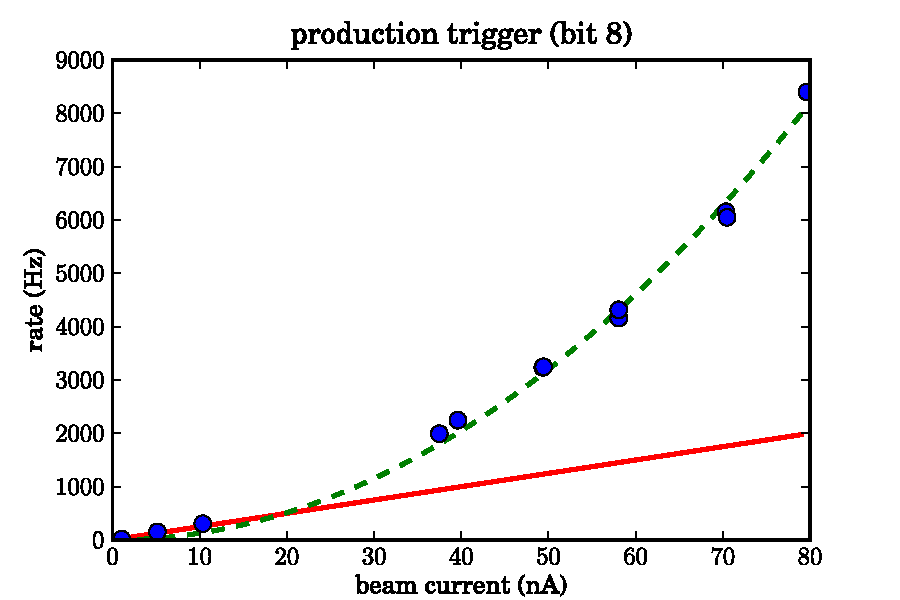
\includegraphics[width=0.7\columnwidth]{\figures/calibration/trigger/trigger_study.pdf}
\caption[Trigger Rate vs. Beam Current]{\label{fig:data.trig.eff}{\coloronline}The production trigger rate (bit 8 in Tables~\ref{tab:data.trig.conf.1} and \ref{tab:data.trig.conf.2}) was measured for various beam currents shown by the blue dots. The rates below 10~nA are roughly linear and are extrapolated via the red solid line to show an estimate of the physical event rate. The actual trigger rate is fitted with a quadratic shown by the green dashed line. By this estimate, the accidental rate is shown to equal the physical event rate at approximately 40~nA. The \g12 experiment was done at 60--65~nA.}
\end{center}\end{figure}

\clearpage

\section{\label{sec:data.calib}Calibrations}

The raw data recorded from the \abbr{CLAS} detector consisted of timing and pulse-height information from the drift-chambers and counters. Timing from all the elements such as wires and \abbr{PMT}s were initially offset from each other. The alignment of these times was accomplished during the reconstruction (see Sec.~\ref{sec:data.cook}) using a database that stored the corrections needed to produce timings that were relative to each other. The \abbr{ADC} pulse height was used by the start counter and time-of-flight to account for the propagation time of the signal, in this case light from the scintillator, to the \abbr{PMT}. Determining these corrections took us a year and three months with a team consisting of two \abbr{JLab} staff scientists, three university professors, two post-docs and four graduate students as listed in Table~\ref{tab:calibrators}. This huge amount effort was neccessary due to the large extent of timing information from such a complex detector.

\begin{table}
\begin{minipage}{\columnwidth}
\begin{center}
\begin{singlespacing}

\caption[\g12 Calibrators]{\label{tab:calibrators}The principal calibrators of the \g12 data set.}

\begin{tabular}{cccp{15ex}}

\hline \hline

name & institution & position & {\raggedright systems and responsibilities} \\

\hline

C.\ Bookwalter & \abbr{FSU}\footnote{Florida State Univ.} & graduate student & \abbr{TOF} \\
P.\ Eugenio & \abbr{FSU} & professor & coordination \\
J.\ Goetz & \abbr{UCLA}\footnote{Univ.\ of California Los Angeles} & graduate student & reconstruction \\
L.\ Guo & \abbr{JLab} & post-doc & coordination \\
V.\ Kubarovsky & \abbr{JLab} & staff scientist & coordination \\
M.\ Paolone & \abbr{USC}\footnote{Univ.\ of South Carolina} & post-doc & \abbr{EC}, \abbr{CC} \\
J.\ Price & \abbr{CSUDH}\footnote{California State Univ.\ Domingus Hills} & professor & coordination \\
M.\ Saini & \abbr{FSU} & graduate student & \abbr{RF}, \abbr{ST}, \abbr{TAG} \\
D.\ Schott & \abbr{FIU}\footnote{Florida International Univ.} & graduate student & \abbr{DC} \\
B.\ Stokes & \abbr{GWU}\footnote{George Washington Univ.} & post-doc & \abbr{DC} \\
A.\ Vlassov & \abbr{ITEP}\footnote{Alikhanov Inst.\ for Theoretical and Experimental Physics} & professor & \abbr{CC} \\
D.\ Weygand & \abbr{JLab} & staff scientist & coordination \\
M.\ Wood & Canisius College & professor & \abbr{EC} \\

\hline \hline

\end{tabular}

\end{singlespacing}
\end{center}
\end{minipage}
\end{table}
\vspace{20pt} % label: tab:calibrators

The general calibration procedure began by determining the timing offset of the systems associated with the event trigger which were the start counter, time-of-flight and tagger. Then, the drift chambers were calibrated for physical alignment and \abbr{TDC} alignment using the zero-field run. The tracks obtained from the \abbr{DC}, along with the \abbr{ADC} signals from the \abbr{ST} and \abbr{TOF} could then be combined to determine the time-walk corrections which were used in subsequent iterations. This process would then be repeated several times until adequate resolutions in the various subsystems were achieved.

We started by aligning all the \abbr{TDC} signals from the scintillators ``paddle to paddle'' in the start counter, tagger and time-of-flight systems. Then, the timings of these systems as a whole were aligned to the radio-frequency time (\abbr{RF}) from the accelerator beam. This \abbr{RF} clock provided the most accurate timing information (approximately 50~ps resolution), and as a result, the likely-hood of choosing the electron in the tagger associated with the photon that interacted in the target to create the event was much greater.

After this initial calibration, several things took place in parallel. First, we determined the positions of the drift-chambers using the zero-field run where all tracks in the \abbr{DC} were straight. Secondly, the start counter and time-of-flight timings were corrected for \emph{time-walk}. This accounted for the time it took from the physical passing of the particle through the scintillator to the final \abbr{TDC} signal that was recorded in the data stream. We used the magnitude of the \abbr{ADC} signal to determine the position of the track inside the scintillator paddle and obtained a correction to the \abbr{TDC} signal. Finally, the electromagnetic calorimeter and the \v{C}erenkov detector signals were aligned in time.

Once this was accomplished, we went back to the alignment of the \abbr{TDC}s in the start counter, tagger and time-of-flight which led to another pass of the calibrations. Each of the steps above contained several iterations themselves. We performed four complete passes, as well as several others where only some systems were corrected, before the data were calibrated well enough to use for physics analysis.

\subsection{\label{sec:data.calib.org}Organization of Calibration Procedure}

During the \g12 run, there were several hardware and software changes which required recalibration of the affected systems. These included changes such as the event trigger or cable lengths from the start counter. Each time a change was made, the subsequent runs were treated separately from the previous runs. A list of runs where such changes were made are listed in Table~\ref{tab:data.cook.org.runs}.

\begin{center}
\begin{singlespacing}
\begin{longtable}{ccp{10em}}
\caption[Calibration Run List]{\label{tab:data.cook.org.runs}A list of the runs which were calibrated for the subsystems: tagger (\abbr{TAG}), start counter (\abbr{ST}), and time-of-flight (\abbr{TOF}). The calibrations were committed into the database for the range starting with the run shown and ending with the run just prior to the next listed run. A brief reason for calibration is given in the last column.} \\

\hline \hline
run & systems affected & reason \\
\hline
\endfirsthead

\multicolumn{3}{l}{\scriptsize continued from previous page.} \\
\hline
run & systems affected & reason\\
\hline
\endhead

\hline
\multicolumn{3}{r}{\scriptsize continued on next page.} \\
\endfoot

\hline \hline
\endlastfoot

56363 & \abbr{TAG, ST, TOF} & start of run \\
56503 & \abbr{ST} & \abbr{ST} adjustment \\
56508 & " & \quad " \quad " \\
56661 & \abbr{TAG, ST, TOF} & trigger and \abbr{ST} changes \\
56663 & " & \quad " \quad " \\
56665 & " & \quad " \quad " \\
56666 & " & \quad " \quad " \\
56670 & \abbr{TAG} & vacuum problem in tagger fixed \\
56673 & \abbr{TAG, ST, TOF} & trigger change \\
56732 & " & \abbr{RF} related problems fixed by Accelerator group \\
56765 & \abbr{TAG} & T20 left \abbr{HV} problem \\
56766 & " & T20 left \abbr{HV} adjusted \\
56782 & \abbr{TAG, ST, TOF} & changes in calibration database \\
56855 & " & \quad " \quad " \\
56923 & " & start of intensity studies \\
57094 & " & changes in calibration database \\
57154 & \abbr{ST} & adjusted \abbr{ST} \abbr{ADC} timing in gate \\

\end{longtable}
\end{singlespacing}
\end{center}
\vspace{20pt} % label:  tab:data.cook.org.runs

\subsection{\label{sec:data.calib.systems}Subsystem Calibrations}

The raw \abbr{TDC} time ($t_\mathtt{TDC}$) from any particular element in the detector is related to the event start time ($t_\mathrm{start}$) by the equation:
\begin{equation}
    t_\mathtt{TDC} = t_\mathrm{start} + t_\mathrm{flight} + t_\mathrm{prop} + t_\mathrm{walk} + t_\mathrm{elec},
    \label{eqn:detector_time}
\end{equation}
where $t_\mathrm{flight}$ is the flight time of the particle from the reaction vertex to the element such as a scintillator paddle or layer in the drift chamber, $t_\mathrm{prop}$ is the propagation time of the signal from the track to the detection electronics (\abbr{PMT}s or readouts at the ends of the wires in the \abbr{DC}), $t_\mathrm{walk}$ (called the \emph{time walk}) is the time it takes the discriminator to recognize the signal as a ``hit,'' and $t_\mathrm{elec}$ is the final electronics delay due to cable lengths and signal relays and is generally a constant for all particles at all momenta. The term of interest, $t_\mathrm{start}$, is by definition the same for all hits in an event, however, it contains an arbitrary offset because it is a function of the trigger and therefore varies from event to event. The three times: $t_\mathrm{flight}$, $t_\mathrm{prop}$ and $t_\mathrm{walk}$ are all functions of the momenta and masses of the particles passing through the detector elements. The approximate magnitudes of each term in Eq.~\ref{eqn:detector_time} is shown in Table~\ref{tab:timings}.

\begin{table}
\begin{minipage}{\textwidth}
\begin{center}
\begin{singlespacing}

\caption[Single Timing Relationships]{\label{tab:timings}Relative timing relationships for the terms of Eq.\ref{eqn:detector_time}. The time ranges are the approximate correction amplitudes applied to the data. The column ``fn.\ of \abbr{PID}'' indicates if the time is dependent on the particle mass or momentum.}

\begin{tabular}{lrcp{25ex}}

\hline \hline

term & approx.\ range & fn.\ of \abbr{PID}? & description \\

\hline

$t_\mathtt{TDC}$ & 0--400~ns & no & recorded time by the electronics \\
$t_\mathrm{start}$ & 0--400~ns & no & event start time \\
$t_\mathrm{flight}$ & 20--50~ns & yes & particle flight time from vertex \\
$t_\mathrm{prop}$ & 0.1--10~ns & yes & signal propagation time \emph{to} electronics \\
$t_\mathrm{walk}$ & 100--400~ps & yes & descriminator response time \\
$t_\mathrm{elec}$ & 0.1--10~ns & no & signal propagation time \emph{in} electronics \\

\hline \hline

\end{tabular}

\end{singlespacing}
\end{center}
\end{minipage}
\end{table}
\vspace{20pt} % tab:timings

The goal of the timing calibrations was to determine all the values in Eq.~\ref{eqn:detector_time} for each detector element as a function of particle momentum, charge and/or mass when neccessary. The actual value of interest is always the flight time of the particles from the reaction vertex to the detector element ($t_\mathrm{flight}$) but the trigger offset inherent in $t_\mathrm{start}$ requires the use of the sum: $t_\mathrm{flight} + t_\mathrm{start}$. Only differences in these times (i.e. between two hits in the detector) were used in this analysis so that the trigger offset could be subtracted.

The two times in Eq.~\ref{eqn:detector_time} that are the most difficult to determine were $t_\mathrm{prop}$ and $t_\mathrm{walk}$. The first of these, the propagation time of the signal from the track to the electronics interface, is a property of the medium such as the gas or scintillator material. For double-ended paddles like in the \abbr{TOF}, this term was eliminated by taking the average of the \abbr{TDC} times from the two sides. The start counter which has \abbr{PMT}s on only one side of the scintillator paddles uses the intersection of the track from the \abbr{DC} information to determine this correction. The \emph{time walk} term ($t_\mathrm{walk}$) is a small ($<5\%$) correction which represents the electronic's interface response time to a physical signal and is a function of the \abbr{ADC} pulse height as discussed below.

Energy calibrations are generally determined using a known event sample within the data. The tagger energy, for example, was calibrated using the exclusive reaction:
\begin{equation}
    \mathrm{\gammaup p \rightarrow p \piup^+ \piup^-}\label{rxn:excl_ppippim}
\end{equation}
where the exclusivity was determined via missing momentum and missing mass cuts using the energy of the tagger hit associated with the event. The photon energy was then adjusted by taking the total energy of the $\mathrm{p \piup^+ \piup^-}$ system using the equation:
\begin{equation}
    E_\mathrm{beam, corrected} = E_\p + E_{\mathrm{\piup^+}} + E_{\mathrm{\piup^-}} - m_\p,
    \label{eqn:ebeam_ppippim}
\end{equation}
where $E_\p$, $E_{\mathrm{\piup^+}}$ and $E_{\mathrm{\piup^-}}$ are the energies of the outgoing particles, and $m_\p$ is the proton (target) mass. The average of at least 10k events per \emph{logical} tagger energy paddle (see Sec.~\ref{sec:clas.tagr}) was used for this correction and the results as a function of the beam energy is shown in Fig.~\ref{fig:data.calib.tag_energy}. The inherent resolution of the tagger paddles for \g12 was approximately 5.6~MeV.

Results from the tagger energy calibration were used to calculate corrections to the momenta of the tracks, the energy corrections were subsequently recalculated. This iterative process was employed several times until the values obtained for both corrections converged. The energy difference between $E_\mathrm{beam, corrected}$ in Eq.~\ref{eqn:ebeam_ppippim} and the energy reported by the tagger is shown in Fig.~\ref{fig:data.calib.ediff_ppippim}.

\begin{figure}\begin{center}
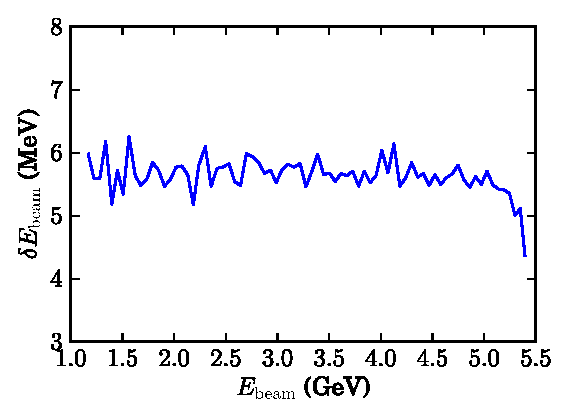
\includegraphics[width=0.55\columnwidth]{\figures/calibration/tagger/tagger_energies.eps}
\caption[\abbr{TAG} Energy Resolution vs.\ Beam Energy]{\label{fig:data.calib.tag_energy}Resolution of the \emph{logical} energy paddles in the tagger. The values were obtained by taking the difference in reported energy between two adjacent paddles. The unevenness can be attributed to overlapping regions of energy counters varying in size and the sagging of the $E$-counter plane\cite{clas.thesis.williams}. An average resolution of 5.6~MeV is indicated by this plot.}
\end{center}\end{figure}

\begin{figure}\begin{center}
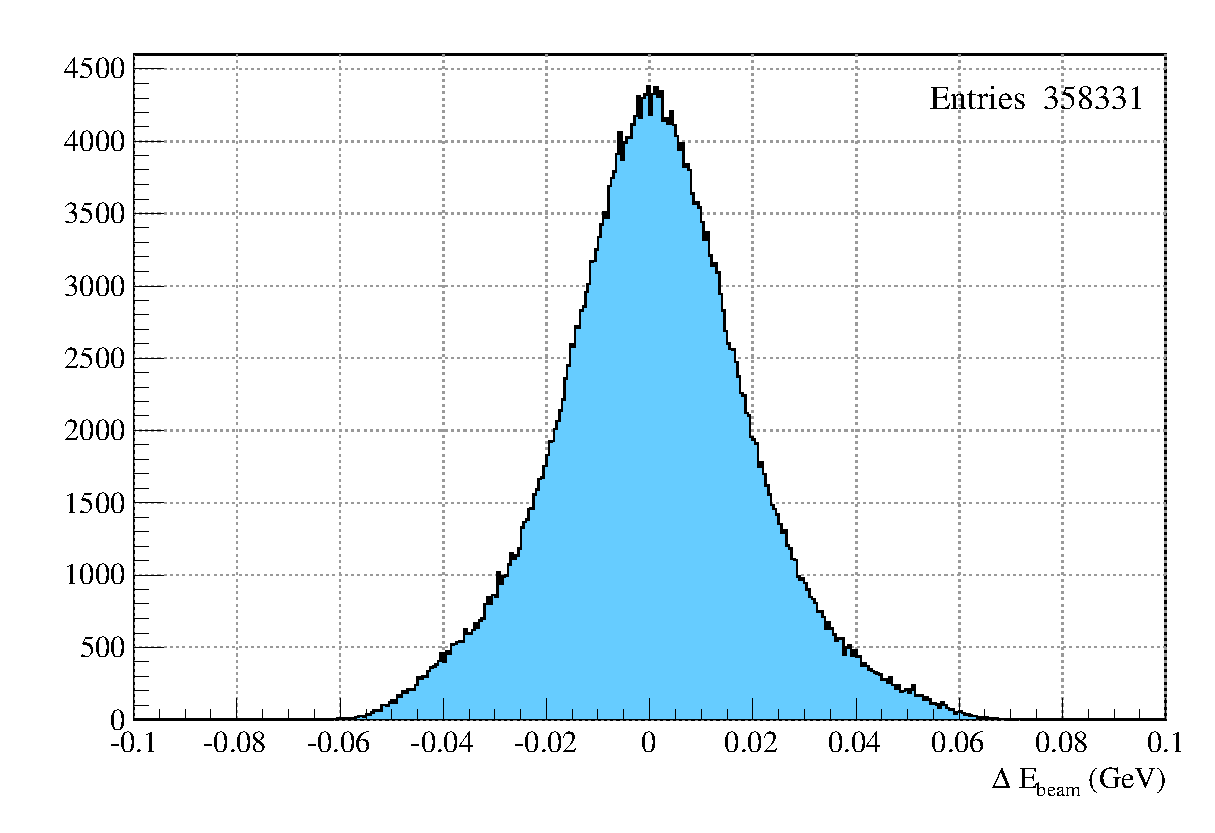
\includegraphics[width=0.7\columnwidth]{\figures/calibration/tagger/ediff_ppippim.eps}
\caption[\abbr{TAG} Energy Resolution, Overall]{\label{fig:data.calib.ediff_ppippim}The energy difference in GeV, between $E_\mathrm{beam, corrected}$ in Eq.~\ref{eqn:ebeam_ppippim}, using the exclusive reaction (\ref{rxn:excl_ppippim}) and the energy reported by the tagger. A Gaussian fit from -0.02 to 0.02~GeV gives a width of $16$~MeV.}
\end{center}\end{figure}

The resolution of the tagger time is approximately 130~ps as shown in Fig.~\ref{fig:data.calib.dttag_ppippim} and this value is used to identify the \abbr{RF} beam-bucket associated with the event. The \abbr{RF} provides the best timing resolution, on the order of a few picoseconds, in \abbr{CLAS} and it is used to calibrate the other systems as described in the sections below.

\begin{figure}\begin{center}
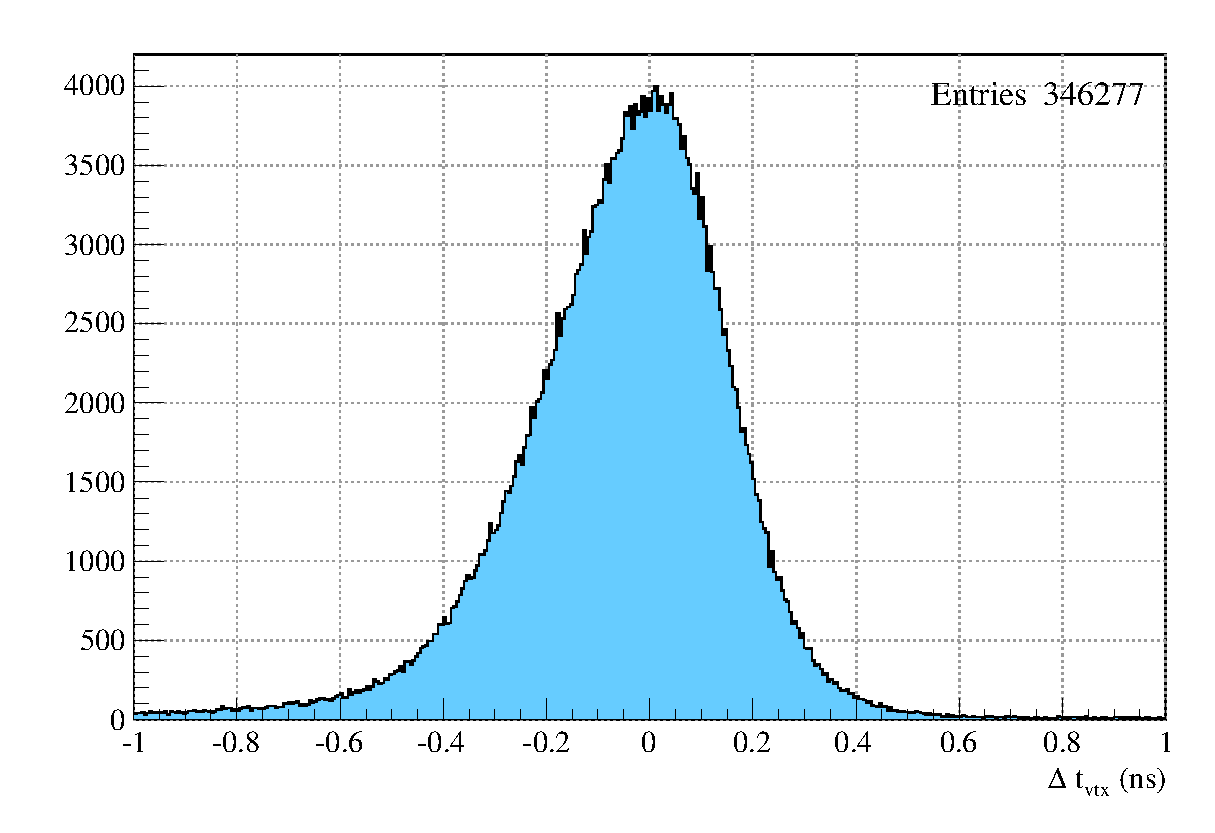
\includegraphics[width=0.7\columnwidth]{\figures/calibration/tagger/dttag_ppippim.eps}
\caption[\abbr{TAG} Timing Resolution]{\label{fig:data.calib.dttag_ppippim}The difference in time between the tagger hit and the nearest \abbr{RF} clock tick using the exclusive reaction (\ref{rxn:excl_ppippim}). A Gaussian fit from -0.2 to 0.2~ns gives a width of $130$~ps.}
\end{center}\end{figure}

The timing of the start counter (\abbr{ST}) was of critical importance for this analysis because it helped determine the tagger hit associated with the physical event. Here again, exclusive $\mathrm{p \piup^+ \piup^-}$ events were used and the tagger hit was matched to the average vertex time measured from these final state particles. The time walk ($t_\mathrm{walk}$) of the signal from the track to the \abbr{PMT} is determined by the equation:
\begin{equation}
    t_\mathrm{walk} = t_0 + \frac{t_{1}}{a - a_0},
    \label{eqn:st_timewalk}
\end{equation}
where $t_0$ and $t_1$ were determined for each paddle from the data. Here, $a$ is the \abbr{ADC} signal and $a_0$ is the \abbr{ADC} pedestal value. The difference in \abbr{ST} vertex time for the tracks and the tagger hit is shown in Fig.~\ref{fig:data.calib.st_dvtime_ppippim} and the final resolution of the \abbr{ST} was approximately 370~ps.


\begin{figure}\begin{center}
\includegraphics[width=0.7\columnwidth]{\figures/calibration/st/dvtime_ppippim.eps}
\caption[\abbr{ST} Timing Resolution]{\label{fig:data.calib.st_dvtime_ppippim}The difference in \abbr{ST} vertex time according to each of the tracks in the exclusive reaction (\ref{rxn:excl_ppippim}) and the tagger hit. A Gaussian fit from -0.5 to 0.5~ns gives a width of $370$~ps.}
\end{center}\end{figure}

The method for determining the \abbr{TOF} resolution is identical to that of the start counter. However, the time walk correction is more sophisticated owing to the finer resolution of the \abbr{TOF}:
\begin{equation}
    t_\mathrm{walk} = \left\{
      \begin{array}{ll}
            b x^{-c}
                &: a < a_1 \\
            \frac{b}{a_1^c}
                \left( b + c \left[ 1
                - \frac{\left( a - a_0 \right)}
                    {a_1 V_T}
                \right] \right)
                &: a \geq a_1
      \end{array}
      \right. ,
\end{equation}
where $t_0$, $b$ and $c$ are constants determined for each \abbr{TOF} paddle and for each calibration run range (see Table~\ref{tab:data.cook.org.runs}), $a$ is the \abbr{TOF} \abbr{ADC} signal, $a_0$ is the \abbr{ADC} pedestal value and $V_T$ is the discriminator threshold value. This equation is essentially a power law below some \abbr{ADC} value $a_1$ and a linear function above, and it has the property of being smooth at this transition point. The difference in vertex times (\abbr{TOF} and \abbr{TAG}) for the (exclusive) $\mathrm{p \piup^+ \piup^-}$ tracks is shown in Fig.~\ref{fig:data.calib.tof_dvtime_ppippim}. The \abbr{TOF} had a timing resolution of approximately 230~ps after all calibrations were completed.

\begin{figure}\begin{center}
\includegraphics[width=0.7\columnwidth]{\figures/calibration/tof/dvtime_ppippim.eps}
\caption[\abbr{TOF} Timing Resolution]{\label{fig:data.calib.tof_dvtime_ppippim}The difference in \abbr{TOF} vertex time according to each of the tracks in the exclusive reaction (\ref{rxn:excl_ppippim}) and the tagger hit. A Gaussian fit from -0.5 to 0.5~ns gives a width of $230$~ps.}
\end{center}\end{figure}

The drift-chamber was calibrated to first-order by aligning the data using the zero-field run where the particles traced a straight line. Once corrected for alignment, fixed delays and track dependent flight times were calculated to obtain the drift time of the signal from the track to each wire, given by\cite{clas.dc.calib}:
\begin{equation}
    t_\mathrm{drift} = t_\mathrm{prop} - t_\mathrm{wire}
    \label{eqn:dc_tdrift}
\end{equation}
where $t_\mathrm{prop}$ is the signal propagation time from Eq.~\ref{eqn:detector_time} and $t_\mathrm{wire}$ is the time the signal took to propagate along the wire from the point of interaction to the electronics. The drift times ($t_\mathrm{drift}$ in Eq.~\ref{eqn:dc_tdrift}) to each wire from the passing particle was then converted to a drift distance and the final tracks were determined by minimizing the absolute value of the residuals, shown in Fig.~\ref{fig:data.calib.residuals_draw}.

\begin{figure}\begin{center}
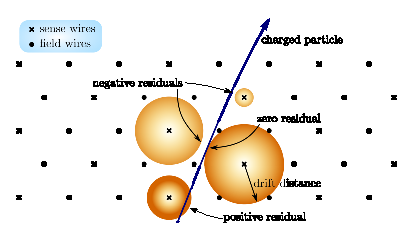
\includegraphics[width=0.85\columnwidth]{\figures/calibration/dc/residuals_drawing.eps}
\caption[\abbr{DC} Residuals Schematic]{\label{fig:data.calib.residuals_draw}Schematic of a track going through five layers of the drift chamber looking down the sense and field wires of the \abbr{DC}. Shown are the residuals obtained from the calculated drift distance, $t_\mathrm{drift}$ in Eq.~\ref{eqn:dc_tdrift}.}
\end{center}\end{figure}

The mean of the residuals is shown in Fig.~\ref{fig:data.calib.dc_res_mean}. The spread from $-50$ to 50~\um\ in the mean contributes to the overall resolution in the drift chambers. The standard deviation of the residuals in the \abbr{DC}, shown in Fig.~\ref{fig:data.calib.dc_res_sig}, was no greater than 380~\um\ for superlayer 6 --- the farthest from the target. These values combine to give a resolution of approximately 430~\um.

The maximum error of the momentum from the \abbr{DC} can be estimated by considering the constant magnetic field approximation where the particle traces a circular arc in region 2. The momentum ($p$) can be calculated from the saggita ($s$), which is described in Fig.\ref{fig:sagitta}, of the track in this region by
\begin{equation}
    p = \frac{\ell^2 q B}{8 s},
    \label{eqn:momentum_saggita}
\end{equation}
where $\ell$ is the length of the cord defined by the arc, $q$ is the charge, and $B$ is the magnetic field. The cord length was approximately 1.5~m, the charge was $\pm e$ and the magnetic field was $\sim 1$~T. If we take the resolution of the saggita ($\delta s$) to be the resolution of the residuals, then the error of the momentum ($\delta p$), which is momentum-dependent, becomes
\begin{equation}
    \delta p = \frac{8 p^2}{\ell^2 q B} \delta s.
    \label{eqn:momentum_saggita_err}
\end{equation}
This gives an approximate resolution of:
\begin{equation}
    \delta p = 0.002~\mathrm{GeV}^{-1} \times p^2.
    \label{eqn:momentum_resolution}
\end{equation}
Therefore, a 2~GeV particle going through the drift chamber should have an approximate resolution of 8~MeV. It is useful to note that this is an estimate on the \emph{maximum} error and that final momentum corrections, which are discussed in Sec.~\ref{sec:analysis.pid}, were done based on particle identification to further improve the resolution in the data.

\begin{figure}\begin{center}
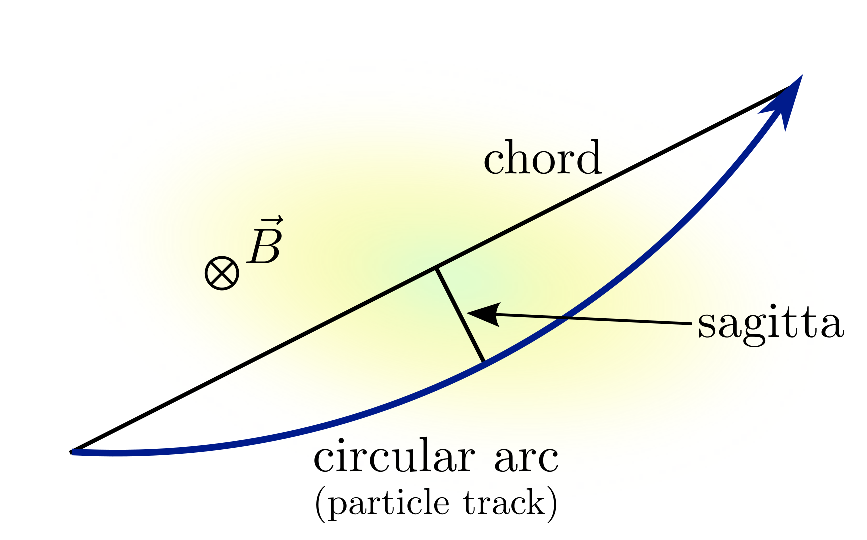
\includegraphics[width=0.45\columnwidth]{\figures/reconstruction/sagitta.eps}
\caption[Saggita of a Circular Arc]{\label{fig:sagitta}The sagitta of a circular arc is the maximum distance between the arc and a given chord. Since charged particles traveling perpendicular to a uniform magnetic field trace a circular path, this is used as an approximation for determining the maximum error of the measured momentum. Shown here is a positively charged particle moving through a uniform magnetic field ($\vec{B}$) going into the page.}
\end{center}\end{figure}

\begin{figure}\begin{center}
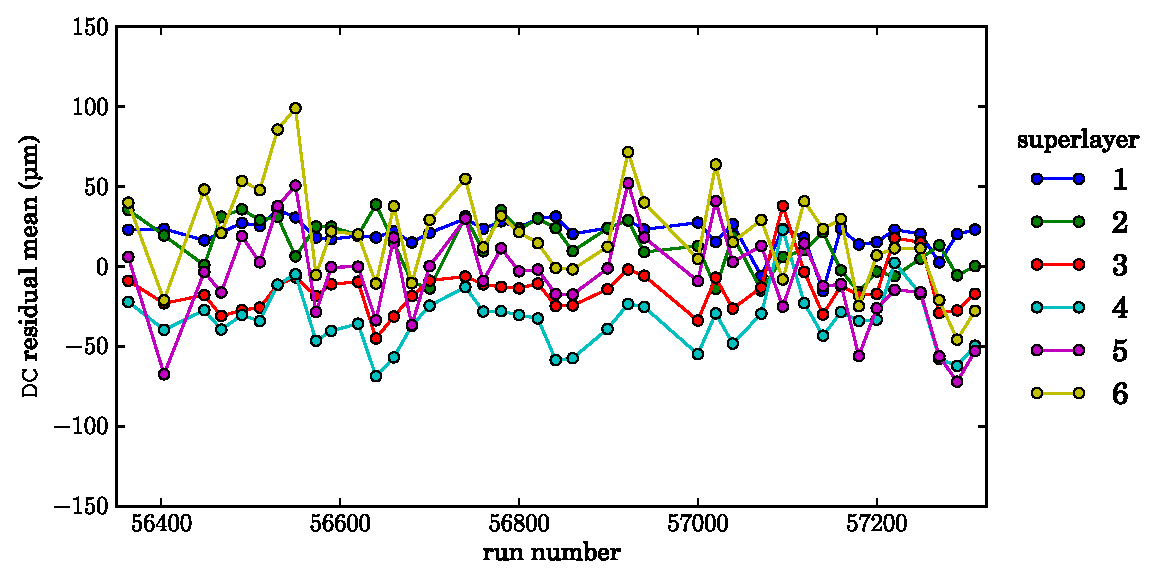
\includegraphics[width=0.85\columnwidth]{\figures/calibration/dc/dc_resid_mean.eps}
\caption[\abbr{DC} Resolution (Residuals, mean)]{\label{fig:data.calib.dc_res_mean}{\coloronline}Mean of residuals in the drift-chamber for each of the six superlayers. A characteristic subset of the good runs listed in Table~\ref{tab:data.cook.prodruns} were used.}
\end{center}\end{figure}

\begin{figure}\begin{center}
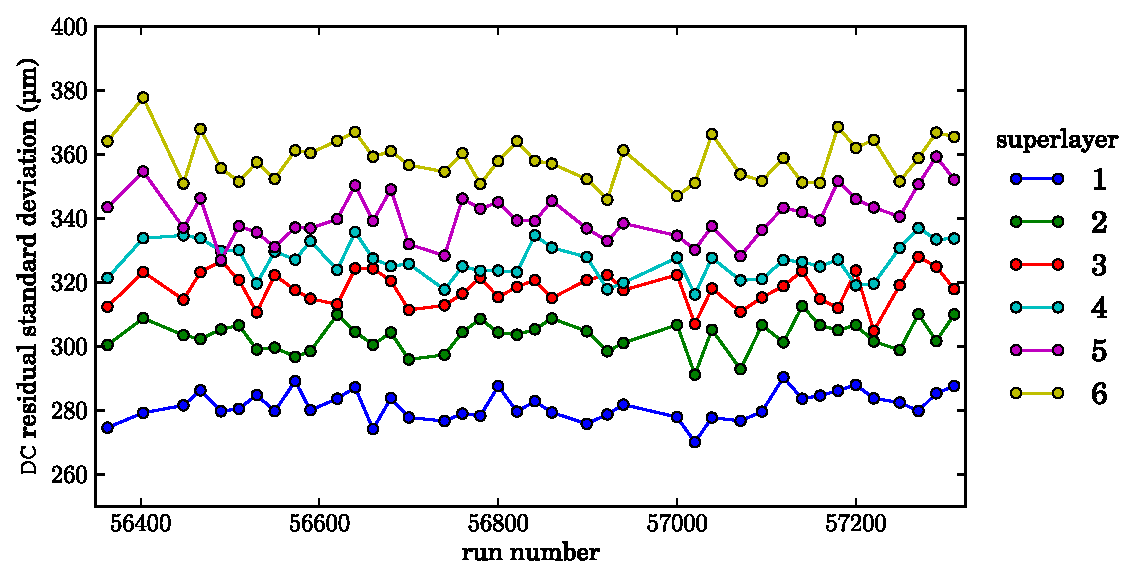
\includegraphics[width=0.85\columnwidth]{\figures/calibration/dc/dc_resid_sigma.eps}
\caption[\abbr{DC} Resolution (Residuals, standard dev.)]{\label{fig:data.calib.dc_res_sig}{\coloronline}Standard deviation of residuals in the drift-chamber for each of the six superlayers. A characteristic subset of the good runs listed in Table~\ref{tab:data.cook.prodruns} were used.}
\end{center}\end{figure}

\clearpage


\section{Raw Data Reconstruction}\label{sec:data.cook}

The process of reconstructing tracks and their subsequent particle identification from raw data is referred to as ``cooking'' and was done by the program \texttt{a1c}\label{abbr:a1c} for \g12. ``Cooking'' is when the information recorded from the various detector subsystems is converted into a form suitable for physics analysis. During cooking, each detector subsystem was calibrated. The ``cooking'' of the \g12 dataset was performed by John Theodore Goetz and is fully documented in~\cite{clas.g12.note} and~\cite{goetz}.

The ``cooking'' process performed by \texttt{a1c} is outlined in Fig.~\ref{fig:data.cook.flowchart}. Initial calibrations are done for each subsystem in each sector the process begins with ``hit-based'' tracking in the \abbr{DC}. ``Hit-based'' tracking requires only the positions of wires registering a hit in a given sector. Adjacent hits in each superlayer are assembled into clusters, and then these clusters are linked in each region to produce track segments. Refer to Fig.~\ref{fig:clas.dc.drift} for an illustration of a track segment. Track segments are linked over the three regions to produce full hit-based trajectories. See Fig~\ref{fig:data.cook.flowchart.hitbased} for a pictorial description of ``hit-based'' tracking. There was an overall failure of events that should have passed ``hit-based'' tracking but failed. This will be discussed fully in Sec.~\ref{sec:analysis.accept.verify}.
%, but can be seen in Fig.~\ref{sec:clas.st.eff} as an overall inefficiency of 3.75\%.

\begin{figure}\begin{center}
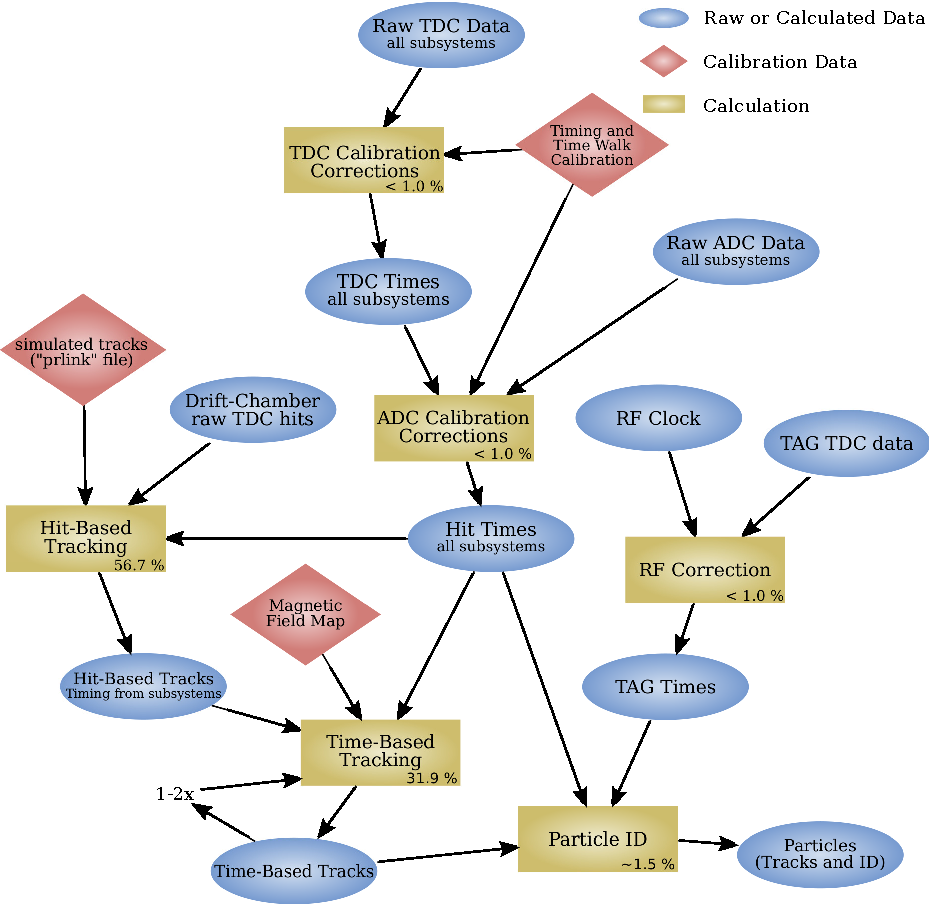
\includegraphics[width=0.92\columnwidth]{\figures/reconstruction/clas6_cooking_diagram_color.pdf}
\caption[Flow chart of the reconstruction process from raw data to identified tracks with momentum]{\label{fig:data.cook.flowchart}Flow chart of the reconstruction process from raw data to identified tracks with momentum. ``Subsystems'' refers to the \abbr{ST}, \abbr{CC}, \abbr{TOF} and the \abbr{EC} detectors. Percentages shown indicate the relative time taken to do the calculations.}
\end{center}\end{figure}

\begin{figure}\begin{center}
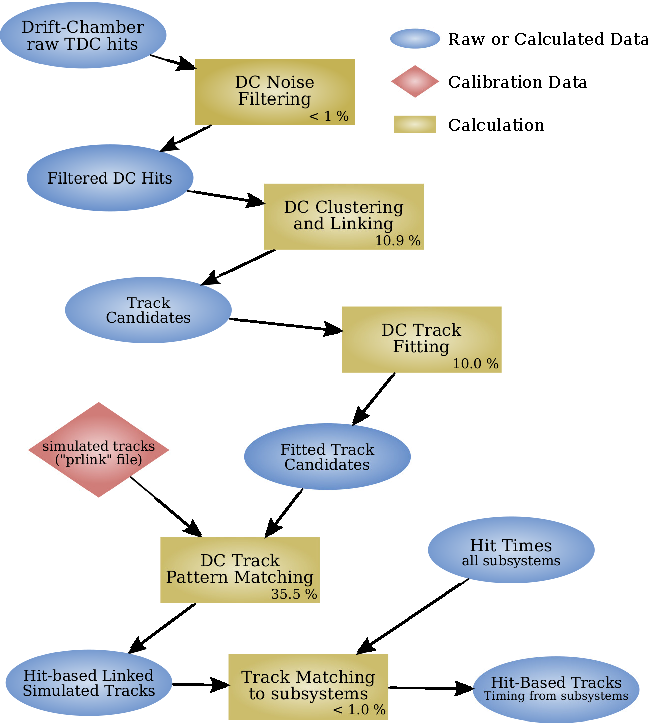
\includegraphics[width=0.7\columnwidth]{\figures/reconstruction/clas6_hitbasedtracking_diagram_color.pdf}
\caption[Flow chart of the hit-based tracking part of the reconstruction]{\label{fig:data.cook.flowchart.hitbased}Flow chart of the hit-based tracking part of the reconstruction shown in Fig.\ref{fig:data.cook.flowchart}. ``Subsystems'' refers to the \abbr{ST}, \abbr{CC}, \abbr{TOF} and the \abbr{EC} detectors. Percentages shown indicate the relative time taken to do the calculations with respect to the full reconstruction.}
\end{center}\end{figure}


After ``hit-based'' tracking is performed, ``time-based'' tracking is performed on the hits obtained from ``hit-based'' track to the appropriate \abbr{TOF} panel. This is done to eliminate noise hits or whole clusters that are not associated with physical tracks. If a hit from ``hit-based'' tracking is found to match a \abbr{TOF} panel, the time measurement from the \abbr{TOF} panel is used to set an upper limit to the time of the drift-chamber hits. With this upper limit known, the \abbr{DC} hits associated with the track are checked individually, where each hit is required to be in increasing time order as the track moves away from the target, any hits or whole clusters not satisfying this requirement are removed. After the removal of the initial bad hits, the track is refit using the remaining hits and the process of removing bad hits is repeated up to two more times to further refine momentum measurements, as well as the measurement of the event vertex, which is determined by the distance of closest approach of the track to the beamline. When the processes of ``time-based'' tracking is finished, all other subsystem information is then added to the tracks properties list. See Fig~\ref{fig:data.cook.flowchart.timebased} for a pictorial description of ``time-based'' tracking. 

During the initial stages of ``time-based'' tracking, a \abbr{ST} signal must be present. This will be discussed in Sec.~\ref{sec:analysis.accept.verify}.  If the track failed due to this error, it usually passed ``time-based'' on the second or third pass of the ``time-based'' tracking if another particle passed ``time-based'' during the initial pass. The average inefficiency for three track events for data was $<0.01$\%
% that there was a random bug in the processing of the \abbr{TDC} element information of \abbr{ST} (\abbr{STN0}) and the \abbr{ADC} element information of \abbr{ST} (\abbr{STN1}) raw data banks. The bug miscalculated the tracks sector exiting the \abbr{ST} even as the hit element of the \abbr{ST} matched that to the track in the \abbr{DC}. This inefficiency can be seen in Fig.~\ref{sec:clas.st.eff}. If the track failed due to this error, it usually passed ``time-based'' on the second or third pass of the ``time-based'' tracking if another particle passed ``time-based'' during the initial pass. The average inefficiency for three track events for data was 0.0125\%

The process of ``cooking'' was performed for Monte-Carlo data for the purpose of verifying the simulation package and the presence of this error and the ``hit-based'' inefficiency is discussed in Sec.~\ref{sec:analysis.accept.verify}.

\begin{figure}\begin{center}
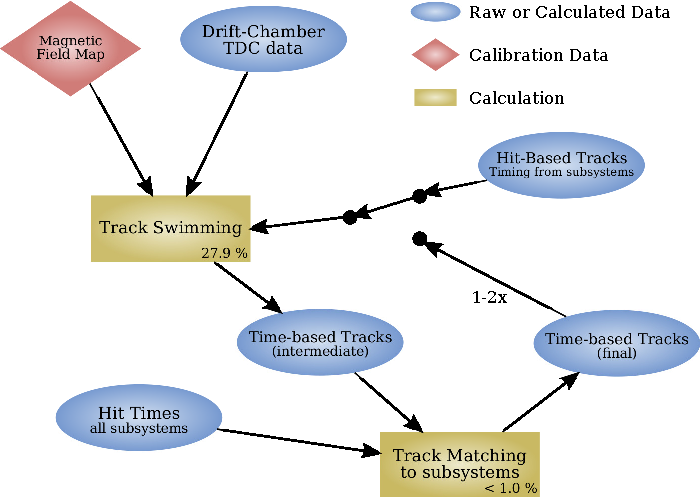
\includegraphics[width=0.8\columnwidth]{\figures/reconstruction/clas6_timebasedtracking_diagram_color.pdf}
\caption[Flow chart of the time-based tracking part of the reconstruction]{\label{fig:data.cook.flowchart.timebased}Flow chart of the time-based tracking part of the reconstruction shown in Fig.\ref{fig:data.cook.flowchart}. ``Subsystems'' refers to the \abbr{ST}, \abbr{CC}, \abbr{TOF} and the \abbr{EC} detectors. The switch indicates that hit-based tracks are input into the swimming calculation, after which the time-based tracks are used creating a feedback loop. Percentages shown indicate the relative time taken to do the calculations with respect to the full reconstruction.}
\end{center}\end{figure}




%The tagger energy was calibrated using the exclusive reaction:
%\begin{align}\label{rxn:excl_ppippim}
%    \mathrm{\gamma p \rightarrow p \pi^+ \pi^-}
%\end{align}
%where the exclusivity was determined via missing momentum and missing mass cuts using the energy of the tagger hit associated with the event. The photon energy was then adjusted by taking the total energy of the $\mathrm{p \pi^+ \pi^-}$ system using the equation:
%\begin{align}\label{eqn:ebeam_ppippim}
%    E_\mathrm{beam, corrected} = E_\p + E_{\mathrm{\pi^+}} + E_{\mathrm{\pi^-}} - m_\p,   
%\end{align}
%where $E_\p$, $E_{\mathrm{\pi^+}}$ and $E_{\mathrm{\pi^-}}$ are the energies of the outgoing particles, and $m_\p$ is the proton (target) mass. The average of at least 10k events per \emph{logical} tagger energy paddle (see Sec.~\ref{sec:clas.tagr}) was used for this correction and the results as a function of the beam energy is shown in Fig.~\ref{fig:data.calib.tag_energy}. The inherent resolution of the tagger paddles for \g12 was approximately 5.6~MeV.
%
%Results from the tagger energy calibration were used to calculate corrections to the momenta of the tracks, the energy corrections were subsequently recalculated. This iterative process was employed several times until the values obtained for both corrections converged. The energy difference between $E_\mathrm{beam, corrected}$ in Eq.~\ref{eqn:ebeam_ppippim} and the energy reported by the tagger is shown in Fig.~\ref{fig:data.calib.ediff_ppippim}.
%
%The resolution of the tagger time is approximately 130~ps as shown in Fig.~\ref{fig:data.calib.dttag_ppippim} and this value is used to identify the \abbr{RF} beam-bucket associated with the event. The \abbr{RF} provides the best timing resolution, on the order of a few picoseconds, in \abbr{CLAS} and it is used to calibrate the other systems as described in the sections below.

\section{Particle Identification}\label{sec:data.pid}

The final procedure is to assign the track a particle mass ($m$). In Sec.~\ref{sec:clas.tof} Eqs.~\ref{eq:beta.cal} and~\ref{eq:mass.cal} explain how the mass of a particle is determined. Fig.~\ref{fig:data.pid} depicts a 2-dimensional plot of the quantities used to determine the particle mass. Once the mass has been determined, particle identification \abbr{PID} is determined by the following criteria;
%Figure~\ref{fig:data.pid} depicts a plot of the quantities used to determine the particles mass,
\begin{align}\label{list:pid}
\abbr{PID} =
\begin{cases}
\pi^{\pm}, & \mathrm{if} \  m  <  0.3~\mathrm{GeV} \ \mathrm{and} \  q  \pm \\
K^{\pm}, &  \mathrm{if} \ 0.35 < m  <  0.35~\mathrm{GeV} \ \mathrm{and} \  q  \pm  \\
p^{\pm}, & \mathrm{if \ 0.8 \ < \ }m \mathrm{\ < \ 1.2 \ GeV \  and \  q  \pm} \\
d, & \mathrm{if \ 1.75 \ < \  }m  \mathrm{\ < \ 2.2 \ GeV } \\
\end{cases}
\end{align}
The events which had particles falling within the undefined regions of the cuts listed in Eq.~\ref{list:pid} were deemed ambiguous events and were given the \abbr{PID} of \emph{``unknown''}. For the analysis of this work, \emph{``unknown''} were used and is described in Sec.~\ref{sec:analysis}

Since tracking began after the particle had already traversed through the target and \abbr{ST}, the measured momentum determination was decreased by the ``energy-loss'' the particle underwent before entering the Region 1 \abbr{DC}. These effects were taken into account as part of the ``energy-loss'' correction during the analysis phase as discussed in Sec.~\ref{sec:analysis.corrections.eloss}.  Once particle identification is completed on the reconstruction level, all relevant information about the particle is collected into the event of occurrence and this information is written in \abbr{BOS} format. There are multiple methods for analyzing \abbr{BOS} format, the chapter~\ref{sec:analysis} will discuss the method used in this analysis. 
%
\begin{figure}\begin{center}
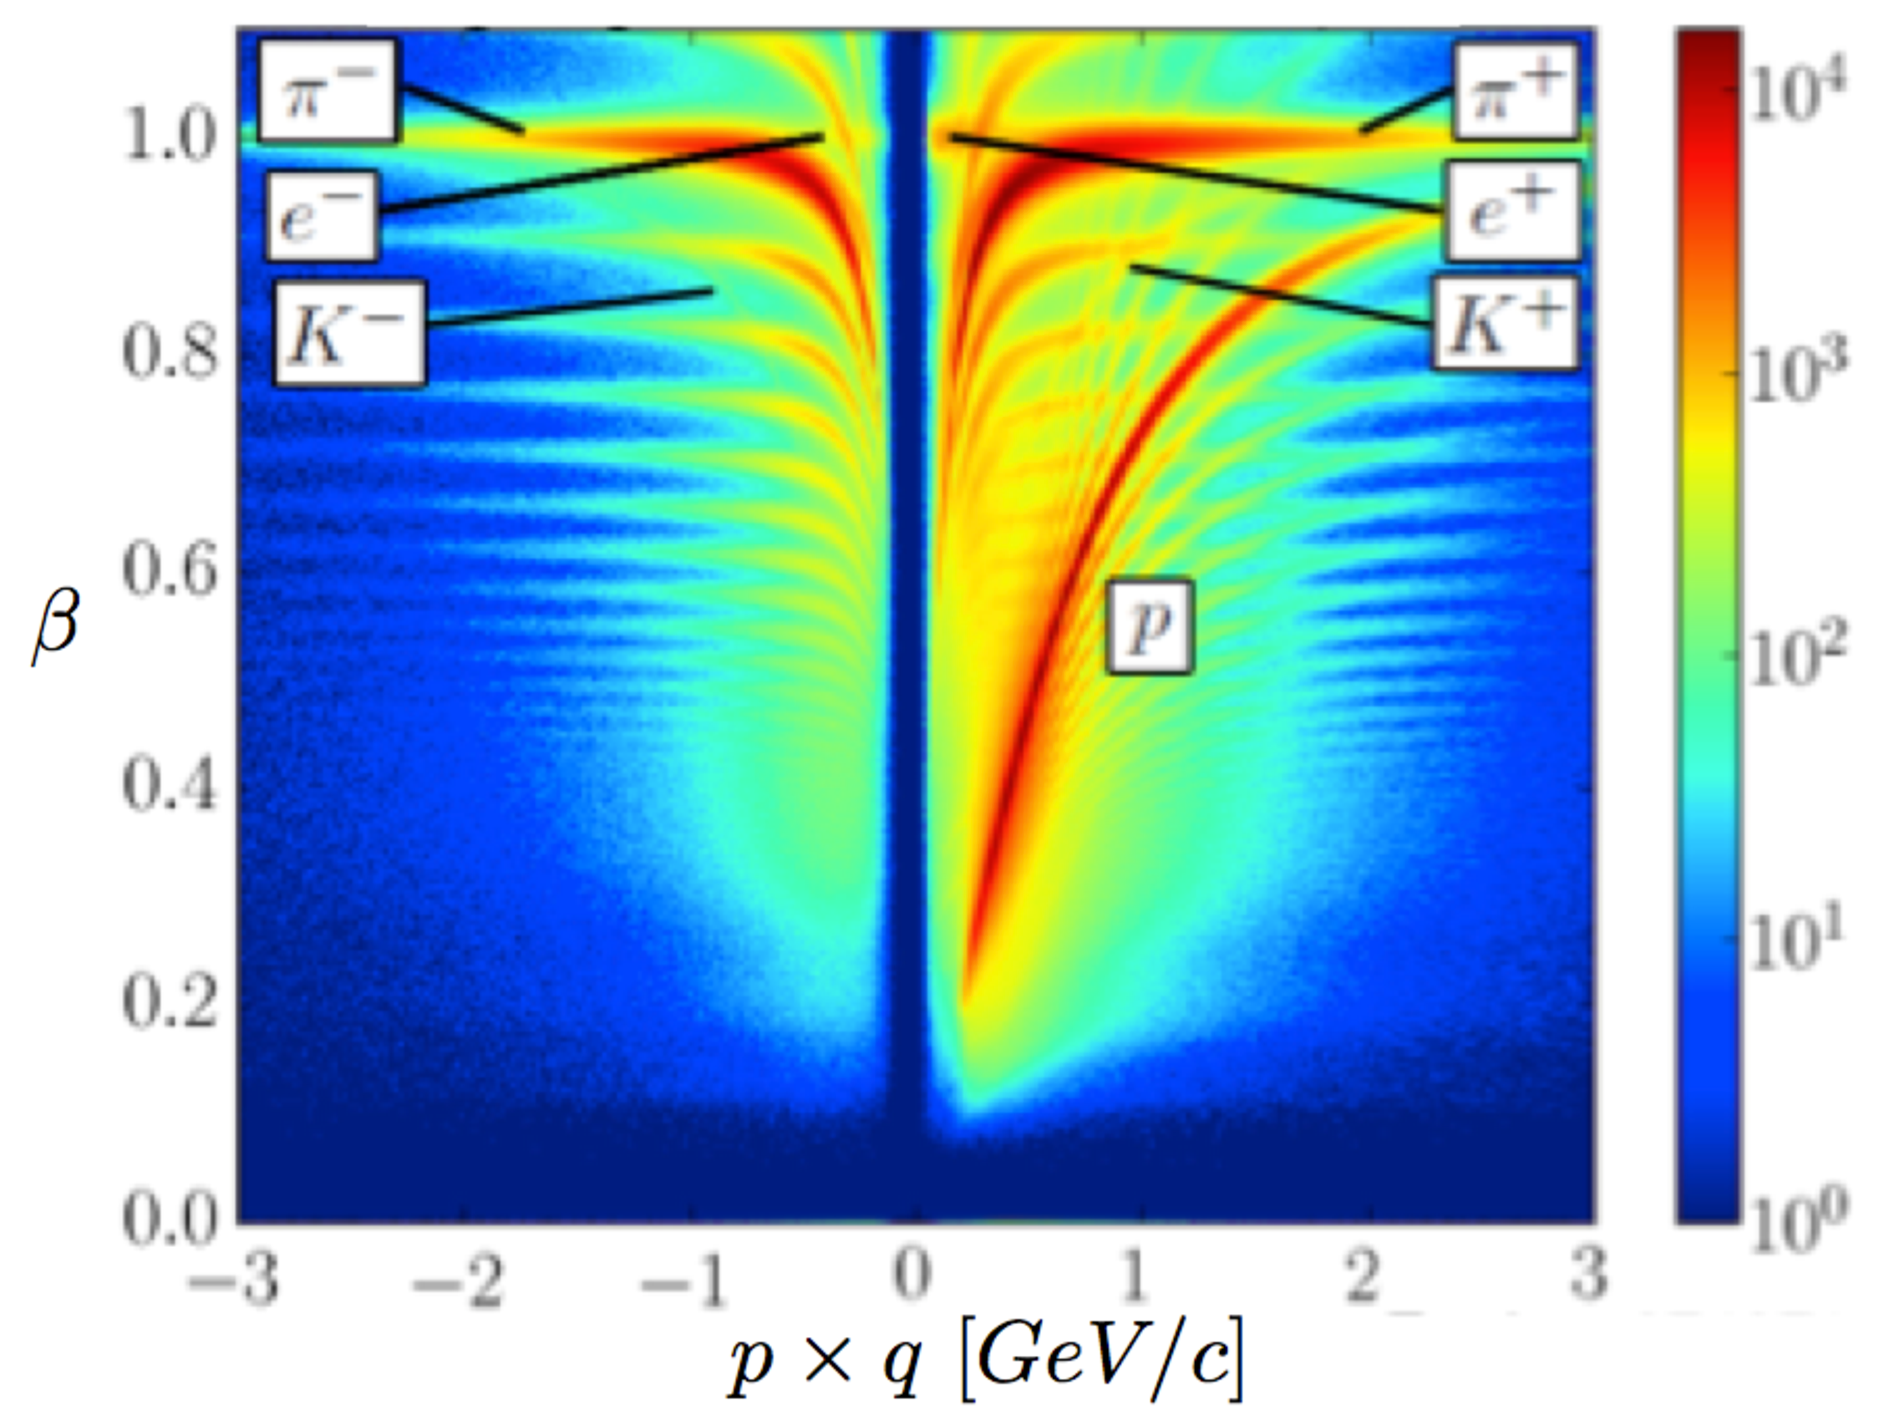
\includegraphics[width=0.9\columnwidth,height=\hfigheight]{\figures/hall-b/g12_pid.pdf}
\caption[$\beta$ vs. mometum(p)$\times$charge(q) for run 56855]{\label{fig:data.pid} $\beta$ vs. mometum(p)$\times$charge(q) for run 56855. This plot is a graphical representation of how particle ID assignments are made in CLAS reconstruction. The ``ribs" seen represent tracks that were ``out-of-time" with a incident photon. Image Source:~\cite{bookwalter}}
\end{center}\end{figure}

%%%\input{data/resolution}
%\section{\label{sec:data.variables}Description of Variables Used in Analysis}

The variables discussed in this work are based on the values stored in the reconstructed \abbr{BOS} banks. Enumerated here are all the values used in this analysis. The structure of the data consists of any number of banks which have a three or four letter identifier with a \emph{sector number} which is just an index from one and not to be confused with the \abbr{CLAS} sectors. It does happen occasionally that the bank sector number corresponds to the \abbr{CLAS} sectors but not always. Each bank consists of a specific set of named variables. The list shows the $bank$ name, \abbr{BOS}-$sector$ number, $hit$ number and $variable$ named used in the \abbr{BOS} file: \bank{BANK}{sector}{hit}{variable}. A corresponding variable, as it is used in the equations of this work, follows in parentheses. The $hit$ number is usually zero for banks that occur only once for an event (e.g. the \abbr{HEAD} bank), while in other cases it is an integer ranging from 1 and denoted by $i$ (e.g. the \abbr{TAGR} bank) corresponding to a specific hit in the given \abbr{BOS}-sector or subsystem.

It is important to note that the over-all trigger offset time ($\ttrigoffset$) is not known and varies from event to event. It must be subtracted from any timing calculation made, and this is usually done by considering only differences in time, for example $\ttof - \tst$.

\begin{itemize}
    \item Event ``Header'' Information
    \begin{description}
        \item[\bank{HEAD}{0}{0}{nrun}] The run number of the event. \g12 consists of run numbers from 56363 to 57323. Monte Carlo data is always stored as run number 10.
        \item[\bank{HEAD}{0}{0}{nevent}] The event number which is an integer starting from 1.
    \end{description}
    \item \abbr{RF} Clock
    \begin{description}
        \item[\bank{CL01}{0}{0}{rf2}] ($\trf$) An \abbr{RF} time which sets the position of the 2.004 ns clock ticks with respect to the times reported by the subsystems, the tagger and start counter in particular.
    \end{description}
    \item Photon Tagger
    \begin{description}
        \item[\bank{TAGR}{0}{i}{stat}] The status flag of the \ith\ tagger hit which is an output of the reconstruction program. Only values of 7 (single good tagger hit) and 15 (good tagger hit among other good hits) are taken into consideration.
        \item[\bank{TAGR}{0}{i}{t\_id}] The \abbr{TDC} paddle that triggered the \ith\ tagger hit.
        \item[\bank{TAGR}{0}{i}{e\_id}] The ``logical energy paddle'' of the \ith\ tagger hit which runs from 1 to 767, see Sec.~\ref{sec:clas.tagr}, and defines the energy of the associated photon.
        \item[\bank{TAGR}{0}{i}{ttag}] ($\ttag$) The time in nanoseconds when the photon crossed the center of the target according to the \abbr{TDC} measured for the \ith\ tagger hit. It is relative to all other times in the detector.
        \item[\bank{TAGR}{0}{i}{tpho}] ($\ttagrf$) This is the \abbr{RF}-corrected version of the $\ttag$ variable. It is the time in nanoseconds that the photon crossed the center of the target according to the \ith\ tagger hit. The \abbr{RF} time ($\trf$) is used as a vernier to adjust $\ttag$ to the closest \abbr{RF} time ``bucket.'' The difference ($\ttag - \ttagrf$) is never more than $\pm 1.002$~ns.
        \item[\bank{TAGR}{0}{i}{erg}] ($\ebeam$) This is the energy of the photon as determined by the logical energy paddle associated with the \ith\ tagger hit \emph{at the time of reconstruction}. This is subsequently superceeded by the energy obtained from the tagger energy corrections as discussed in Sec.~\ref{sec:data.calib.systems}.
    \end{description}
    \item Start Counter
    \begin{description}
        \item[\bank{STR}{1}{i}{id}] ($\mathtt{ID}_\mathtt{ST}$) Encoded sector and paddle number for the \ith\ start counter hit:
        \[
            \mathrm{sector} = \mathrm{floor}\left(\frac{\mathtt{ID}_\mathtt{ST}}{100}\right),
        \]
        \[
            \mathrm{paddle} = 4 \times \left(\mathrm{sector} - 1\right) + \mathrm{floor}\left(\frac{\mathtt{ID}_\mathtt{ST}}{10}\right) \% 10
        \]
        where function ``floor'' returns only the integral part of the argument and ``\%'' is the modulus operator.
        \item[\bank{STR}{1}{i}{st\_time}] ($\tst$) Time of the \ith\ start counter hit in nanoseconds:
        \[
            \tst = \Delta\tst + \ttrigoffset,
        \]
        where $\Delta\tst$ is the time the particle traveled from the vertex (the time of the track at the point of closest approach to the beam) to the start counter paddle, and where $\ttrigoffset$ is the over-all trigger offset time for the event.
        \item[\bank{ST1}{0}{i}{adc\_1}] ($\adcst$) The raw \abbr{ADC} value of the \ith\ start counter hit associated with the \ith\ hit in the \abbr{STR} bank, \abbr{BOS}-sector 1.
    \end{description}
    %\item Reconstructed Tracks
    %\begin{description}
    %    \item[\bank{TDPL}{0}{i}{x}]
    %\end{description}
\end{itemize}

